
\section{Statistical Methods}\label{sec:R}
{\small\noindent{\em The first 3 rules of statistics: 'Draw a picture, Draw a picture, Draw a picture.'---Michael Starbird.}  }


R~is a popular
programming/scripting language that is designed to make advanced
statistical analysis accessible.  Because of its ease of use, large user base, and
extensive community development, it is increasingly used by
researchers, statisticians, and data analysts from fields as varied as
economics, machine learning, pharmaceuticals, and finance.  The yearly
useR! conference boasts a sponsor list that includes such diverse
companies as Google, American Credit Acceptance, and the American
Statistical Association.  Virtually all of the most
influential and popular statistical and machine learning algorithms,
including Boosting, the LASSO, and random forests, have associated R
packages, often written by the inventors of the algorithms.  Although
it is difficult to obtain an exact number of R~users, a New York Times
article from 2009 estimated that there are at least 250,000 active R
users, with the number rising each year.  The RStudio company
develops a variety of software technologies, including an integrated
development environment (IDE) and server-side support for running R
programs remotely, that combine to make R~a painless and appealing
programming environment.  Finally, an increasing number of industrial actors, including
Oracle and Revolution Analytics, have begun offering support for R,
helping it gain industrial users.  R~therefore encompasses all the
necessary statistical models for morphometry, linear mixed effects
modeling and machine learning---supplemented with ANTs, we also gain
the necessary image processing core.


\begin{figure}{t}
\begin{center}
  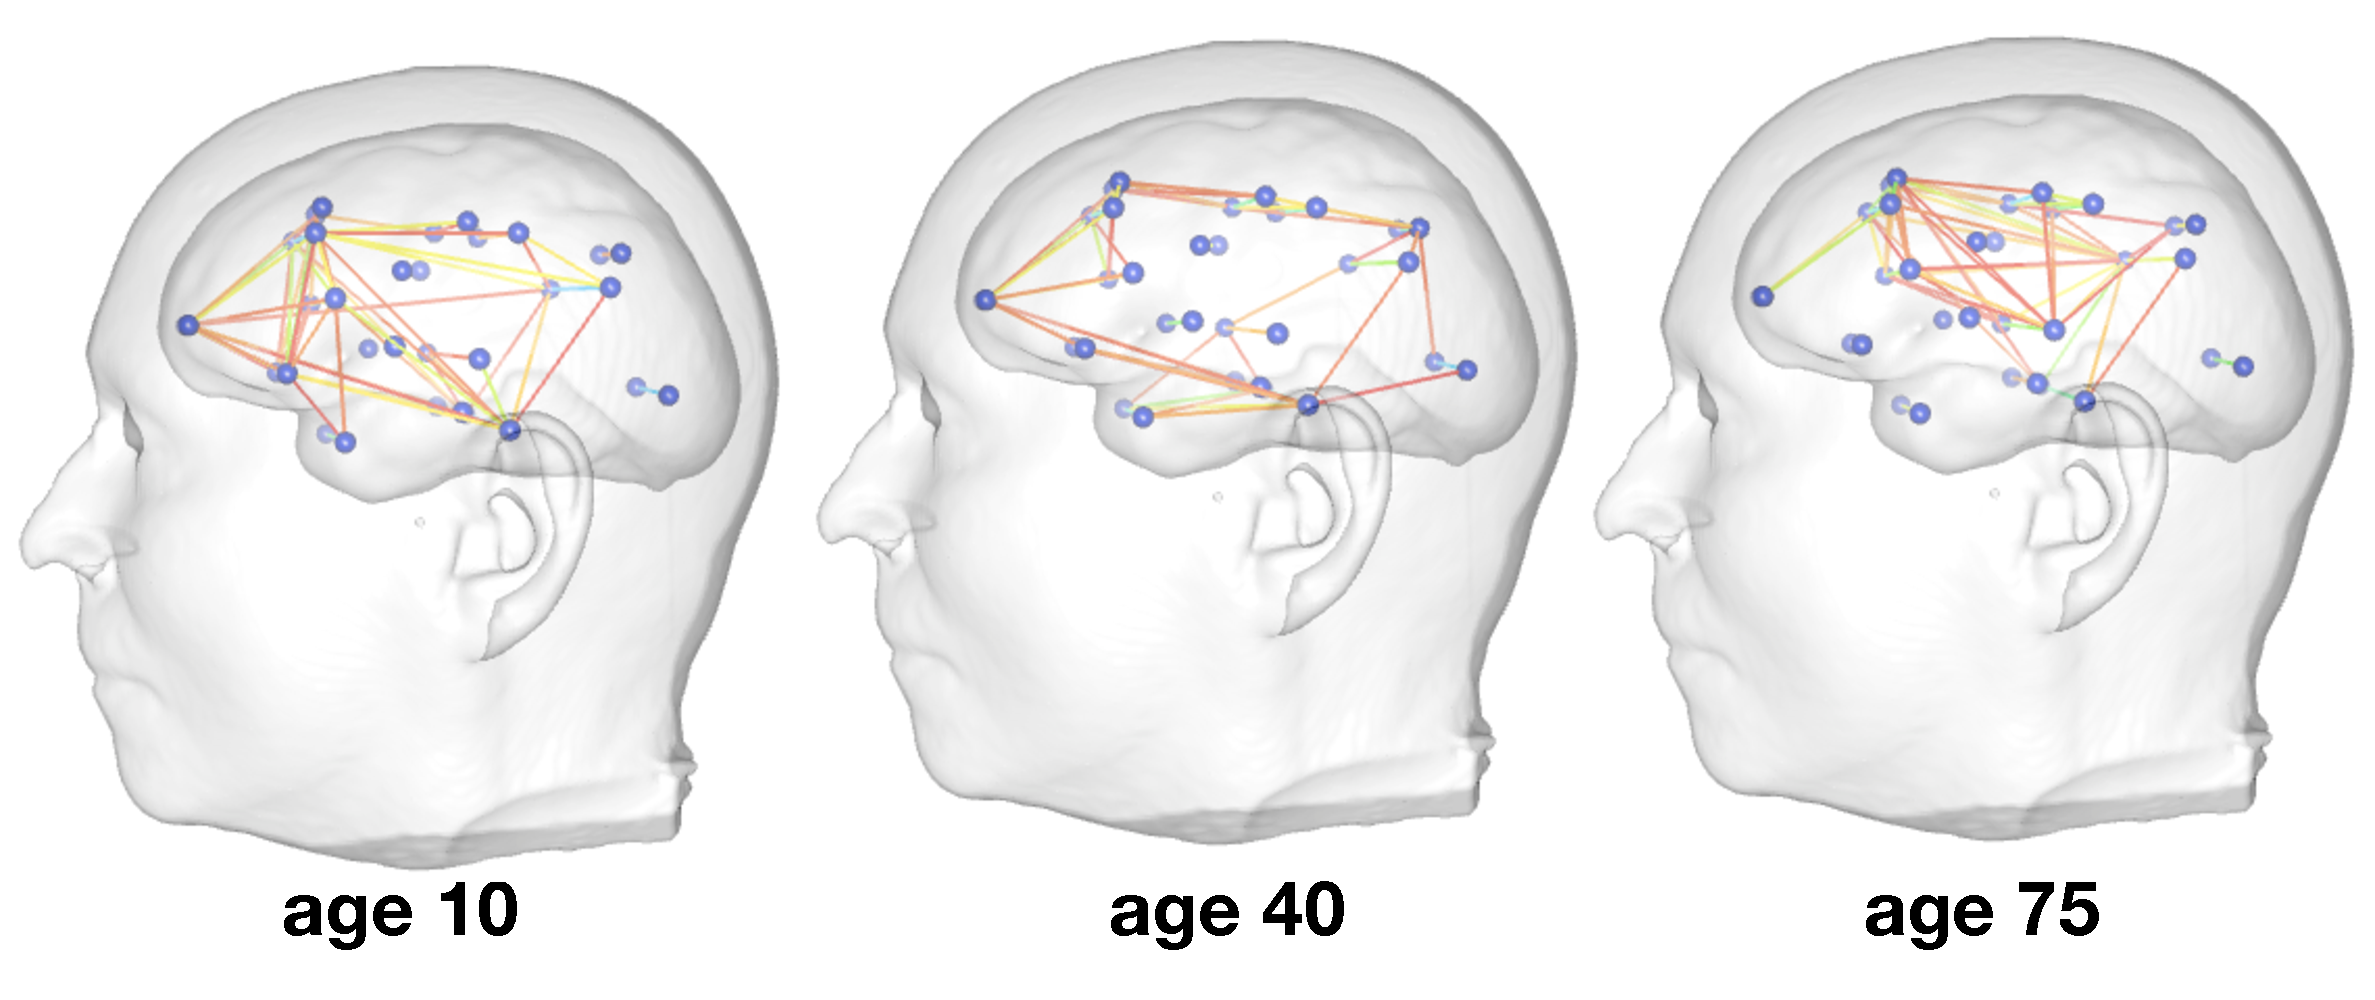
\includegraphics[width=0.9\textwidth]{figs/connx_age}
\end{center}
\caption{ANTsR connectivity analysis shows significant aging effects
  across structural brain networks (n=1200, from public IXI, OASIS, NKI datasets).}\label{fig:cnx}
\end{figure}

When combined with the image processing utilities available in ANTs, R provides a convenient and powerful interface for performing common statistical analyses of imaging data.  In addition, R's standardized syntax minimizes the learning curve for performing a wide variety of different analyses.  The basic form of a statistical model in R is 
\begin{equation}
\text{Outcome} \approx \text{Predictor 1} + \text{Predictor 2} + \text{Predictor 3} + ...
\label{eqn:r_syntax}
\end{equation}
Factor and continuous variable predictors can be combined seamlessly, and a wide variety of model types, including linear models with Gaussian noise, logistic, and Poisson models are available.  When performing a region-of-interest (ROI)-based analysis of the relationship between imaging data and cognition, one typically averages the voxel values within a given ROI and then tests the averaged values against a predictor.  In R syntax, this is written as 
\begin{equation}
\text{ROI value} \approx \text{cognition} + \text{nuisance demographic variables}. 
\label{eqn:ROI}
\end{equation}
Given R's unified interface, conducting voxel-wise morphometric studies of cortical thickness or fractional anisotropy (FA) are similarly easy, with the only difference from Equation \ref{eqn:ROI} being that instead of the ROI value, the original voxel thickness or FA values are provided.  

ANTsR also enables more sophisticated functional studies.  ANTs provides utilities for all necessary preprocessing of time-series data, including motion correction, detrending, and noise reduction (CompCor).  Due to the ease of using factorial predictors in R, task-based fMRI images can be described using the same syntax: 
\begin{equation}
\text{Preprocessed fMRI data} \approx \text{Presence of task} + \text{nuisance regressors}.
\label{eqn:fmri}
\end{equation}
The flexibility of R's linear model functionality also makes tasks that are not typically thought of as regression problems easy to perform.  For example, partial volume corrections in cerebral blood flow (CBF) measurements are often performed using correction equations that can be written as a linear model: 
\begin{equation}
\text{CBF} \approx \text{Percent gray matter} + \text{Percent white matter} + \text{Percent CSF}
\end{equation}
Taking the residual of this model (i.e., the portion of CBF that is not explained by the tissue distribution within a given voxel) is equivalent to performing a partial volume correction.  Once corrected for partial volume effect, the data can be processed using the same method as Equation \ref{eqn:fmri}. 

\begin{figure}
\centering
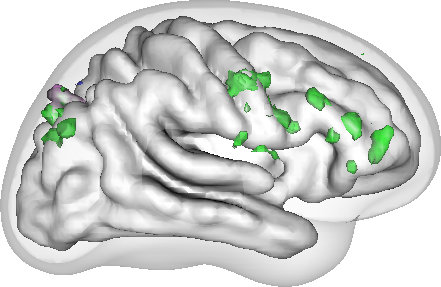
\includegraphics[width=5cm]{figs/bntrenderLateral1.png}
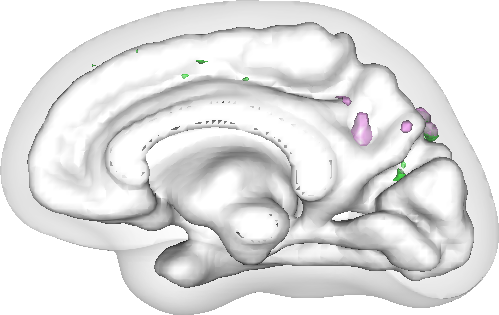
\includegraphics[width=5cm]{figs/bntrenderSagittal1.png}
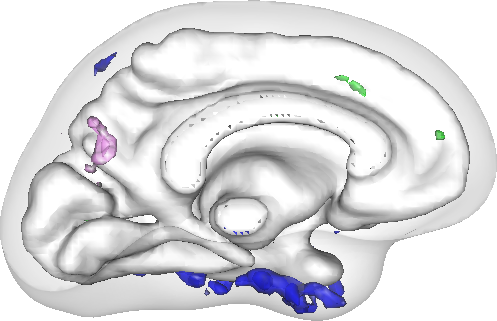
\includegraphics[width=5cm]{figs/bntrenderSagittal2.png}
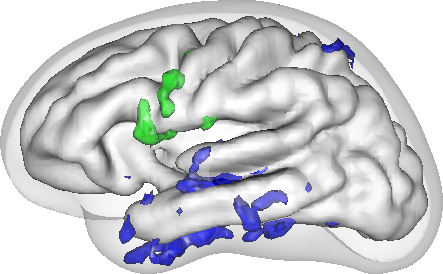
\includegraphics[width=5cm]{figs/bntrenderLateral2.png}
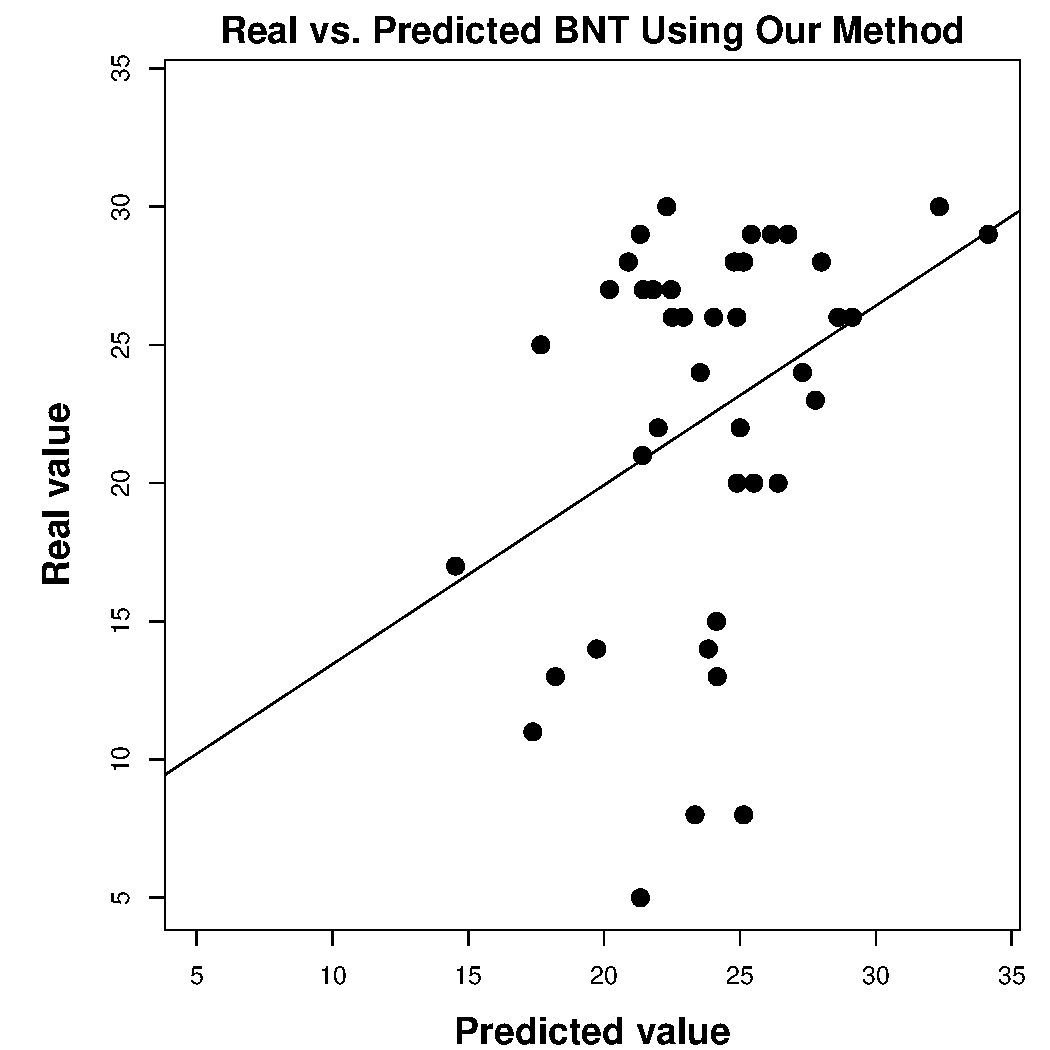
\includegraphics[width=7cm]{figs/predicted_bnt.pdf}
\caption{A demonstration of how ANTsR can be used to find regions that are predictive of performance on the Boston Naming Test.  These regions were found in a training set of data, and then used to predict performance in a testing set.  Predictions on unseen data are seen in the scatterplot.}
\label{fig:bnt}
\end{figure}

In addition to performing standard correlation studies, R provides powerful tools for more rigorous model evaluation, including cross-validation and bootstrapping, and using predetermined coefficients to predict an outcome on unseen data.  Predicting outcomes on data not used for construction of a model is crucial for verifying a model's generalizability and minimizing the possibility of overfitting.  In addition, the root mean square error and similar metrics provide interpretable and intuitively meaningful measures of how well a model matches the data.  Figure \ref{fig:bnt} shows how these techniques can be used to identify regions that are predictive of performance on the Boston Naming Test. 